\documentclass{standalone}
\usepackage{tikz}
\usetikzlibrary{shapes.geometric, arrows.meta}

\tikzset{
  node distance=2cm,
  startstop/.style={rectangle, rounded corners, minimum width=3cm, minimum height=1cm,text centered, draw=black, fill=red!30},
  process/.style={rectangle, minimum width=3cm, minimum height=1cm, text centered, draw=black, fill=orange!30},
  decision/.style={diamond, minimum width=3cm, minimum height=1cm, text centered, draw=black, fill=green!30},
  arrow/.style={thick,->,>=stealth}
}

\begin{document}

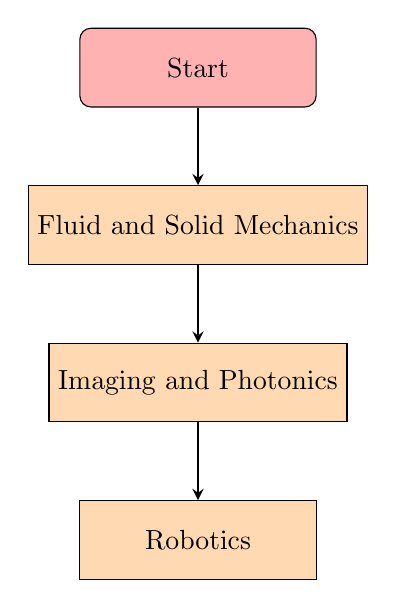
\begin{tikzpicture}[node distance=2cm]

\node (start) [startstop] {Start};
\node (fluid_solid_mechanics) [process, below of=start] {Fluid and Solid Mechanics};
\node (imaging_photonics) [process, below of=fluid_solid_mechanics] {Imaging and Photonics};
\node (robotics) [process, below of=imaging_photonics] {Robotics};

\draw [arrow] (start) -- (fluid_solid_mechanics);
\draw [arrow] (fluid_solid_mechanics) -- (imaging_photonics);
\draw [arrow] (imaging_photonics) -- (robotics);

\end{tikzpicture}

\end{document}